\documentclass{beamer}

\usetheme{Madrid}
\usecolortheme{default}

\usepackage[utf8]{inputenc} % standard encoding since 2018 (can be commented out?)
\usepackage[T1]{fontenc} % absolutely critical for *hyphenation* of words with non-ASCII letters.

% Suggested packages:
\usepackage{microtype}  % towards typographic perfection...
\usepackage{inconsolata} % nicer font for code listings. (Use \ttfamily for lstinline bastype)

% Use package babel for English or Estonian 
% If you use Estonian make sure that Estonian hyphenation is installed 
% - hypen-estonian or eehyp packages
\usepackage[estonian, english]{babel} %the thesis is in Estonian
%\usepackage[english, estonian]{babel} %the thesis is in Estonian

% Change Babel document elements 
\addto\captionsestonian{%
  \renewcommand{\refname}{Viidatud kirjandus}%
  \renewcommand{\appendixname}{Lisad}%
}

% General packages for math in general, theorems and symbols 
% Read ftp://ftp.ams.org/ams/doc/amsmath/short-math-guide.pdf for further information
\usepackage{amsmath} 
\usepackage{amsthm}
\usepackage{amssymb}

% Print a dot instead of colon in table or figure captions
\usepackage[labelsep=period]{caption}

% Packages for building tables and tabulars 
\usepackage{array}
\usepackage{tabu}   % Wide lines in tables
\usepackage{xspace} % Non-eatable spaces in macros

% Including graphical images and setting the figure directory
\usepackage{graphicx}
\graphicspath{{joonised/}}

% Packages for getting clickable links in PDF file
% \usepackage{hyperref}
% \usepackage[hidelinks]{hyperref} %hide red (blue,green) boxes around links
% \usepackage[all]{hypcap}

\usepackage{float}

% Packages for defining colourful text together with some colours
\usepackage{color}
\usepackage{xcolor} 
%\definecolor{dkgreen}{rgb}{0,0.6,0}
%\definecolor{gray}{rgb}{0.5,0.5,0.5}
\definecolor{mauve}{rgb}{0.58,0,0.82}

% Standard package for drawing algorithms
% Since the thesis in article format we must define \chapter for
% the package algorithm2e (otherwise obscure errors occur) 
\let\chapter\section
\usepackage[ruled, vlined, linesnumbered]{algorithm2e}

% Fix a  set of keywords which you use inside algorithms
\SetKw{True}{true}
\SetKw{False}{false}
\SetKwData{typeInt}{Int}
\SetKwData{typeRat}{Rat}
\SetKwData{Defined}{Defined}
\SetKwFunction{parseStatement}{parseStatement}

% Nice todo notes
\setlength {\marginparwidth }{2cm}
\usepackage{todonotes}

% comments and verbatim text (code)
\usepackage{verbatim}

% Obscure packages to write logic formulae and program semantics
% Unless you do a thesis on program semantics or static code analysis you do not need that
% http://logicmatters.net/resources/ndexamples/proofsty3.html <= writing type rules => use semantic::inference
% ftp://tug.ctan.org/tex-archive/macros/latex/contrib/semantic/semantic.pdf
\usepackage{proof}
\usepackage{semantic} 
\setlength{\inferLineSkip}{4pt}
\def\predicatebegin #1\predicateend{$\Gamma \vdash #1$}

% If you really want to draw figures in LaTeX use packages tikz or pstricks
% However, getting a corresponding illustrations is really painful  

% Define your favorite macros that you use inside the thesis
% Name followed by non-removable space
\newcommand{\proveit}{ProveIt\xspace}

% Macros that make sure that the math mode is set
\newcommand{\typeF}[1]{\ensuremath{\mathsf{type_{#1}}}\xspace}
\newcommand{\opDiv}{\ensuremath{\backslash \mathsf{div}}\xspace} 

% Define statistical operators here!
\DeclareMathOperator*{\MEAN}{\mathbf{E}}
\DeclareMathOperator*{\VARIANCE}{\mathbf{D}}
\newcommand{\mean}[1]{\MEAN\left[#1\right]}
\newcommand{\variance}[1]{\VARIANCE\left[#1\right]}
\newcommand{\prob}[1]{\Pr\left[#1\right]}

% Define classifier metrics here
\newcommand{\accuracy}{Acc}
\newcommand{\precision}{Prec}
\newcommand{\recall}{Rec}

%------------------------------------------------------------
%This block of code defines the information to appear in the
%Title page
\title{Masinõppe mudelite hindamine väheste märgenditega andmetel}

% \subtitle{A short story}

% \author[Arthur, Doe] % (optional)
% {A.~B.~Arthur\inst{1} \and J.~Doe\inst{2}}
\author{Mart-Mihkel Aun}

% \institute[VFU] % (optional)
% {
%   \inst{1}%
%   Faculty of Physics\\
%   Very Famous University
%   \and
%   \inst{2}%
%   Faculty of Chemistry\\
%   Very Famous University
% }

\date{Juuni 2023}

%End of title page configuration block
%------------------------------------------------------------

\begin{document}

\selectlanguage{estonian}

\frame{\titlepage}

\section{Taust}

\begin{comment}
    1) sissejuhatus, eesmärgi ja uurimisülesande kirjeldus, ülevaade töö struktuurist,
    2) ülevaade meetodist, lähenemisest, hüpoteesidest,
    3) töö käik,
    4) tulemuste esitlus,
    5) järeldused, kokkuvõte.
\end{comment}

%---------------------------------------------------------
\begin{frame}{Motivatsioon}
    \begin{table}[H]
        \caption{Pildi klassifitseerimine MNIST testvalimil}
        \begin{tabular}{c|c|>{\onslide<2->}c<{\onslide}}
            Meetod              & Õigsus     & Viga           \\ \hline
            EnsNet              & $0{,}998$  & $\pm 0{,}0009$ \\
            CNN                 & $0{,}9969$ & $\pm 0{,}0011$ \\
        	SVM                 & $0{,}9944$ & $\pm 0{,}0015$ \\
        	K-Nearest Neighbors & $0{,}9948$ & $\pm 0{,}0015$ \\
        	Random Forest       & $0{,}972$  & $\pm 0{,}0034$ \\
            Linear Classifier   & $0{,}924$  & $\pm 0{,}0056$ \\
        \end{tabular}
    \end{table}

    \centering
    \tiny{\url{https://paperswithcode.com/sota/image-classification-on-mnist}}
    \tiny{\url{https://en.wikipedia.org/wiki/MNIST_database#Classifiers}}
\end{frame}
%---------------------------------------------------------

%---------------------------------------------------------
\begin{frame}{Veahinnangud}
    \begin{columns}
        \column{0.8\textwidth}
        \begin{figure}[H]
            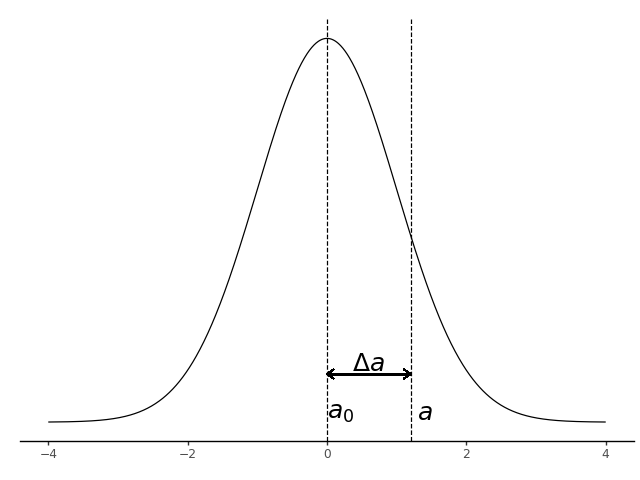
\includegraphics[width=0.8\textwidth]{absoluutne_viga.png}
        \end{figure}

        \column{0.2\textwidth}
        \begin{equation*}
            \Delta a = a - a_0
        \end{equation*}

        \begin{equation*}
            \delta a = \frac{a - a_0}{a_0}
        \end{equation*}
    \end{columns}
\end{frame}
%---------------------------------------------------------

%---------------------------------------------------------
% \begin{frame}{Usaldusintervallid}
%     \begin{columns}
%         \column{0.8\textwidth}
%         \begin{figure}[H]
%             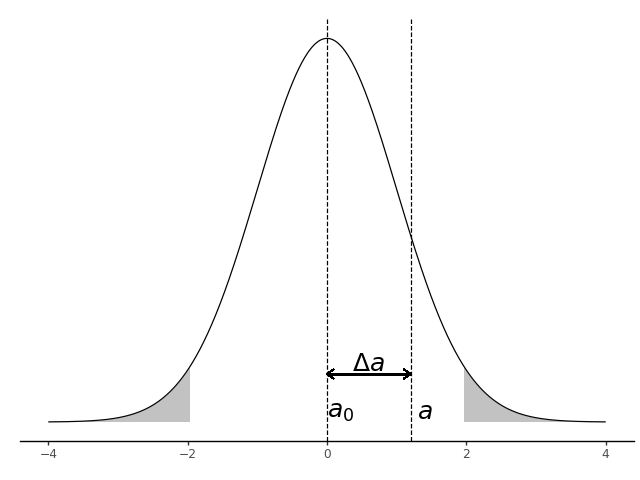
\includegraphics[width=0.8\textwidth]{absoluutne_viga_usaldusintervallid.png}
%         \end{figure}
% 
%         \column{0.2\textwidth}
%         \begin{equation*}
%             \Delta a = a - a_0
%         \end{equation*}
% 
%         \begin{equation*}
%             \delta a = \frac{a - a_0}{a_0}
%         \end{equation*}
%     \end{columns}
% \end{frame}
%---------------------------------------------------------

\section{Kvaliteedimõõtude veahinnangud}

%---------------------------------------------------------
\begin{frame}{Kvaliteedimõõdud}
    \begin{figure}[H]
        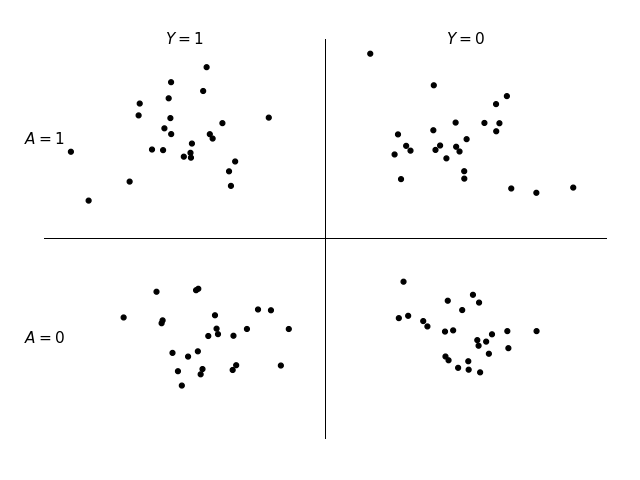
\includegraphics[width=0.8\textwidth]{segadusmaatriks.png}
    \end{figure}
\end{frame}
%---------------------------------------------------------

%---------------------------------------------------------
\begin{frame}{Õigsus}
    \begin{figure}[H]
        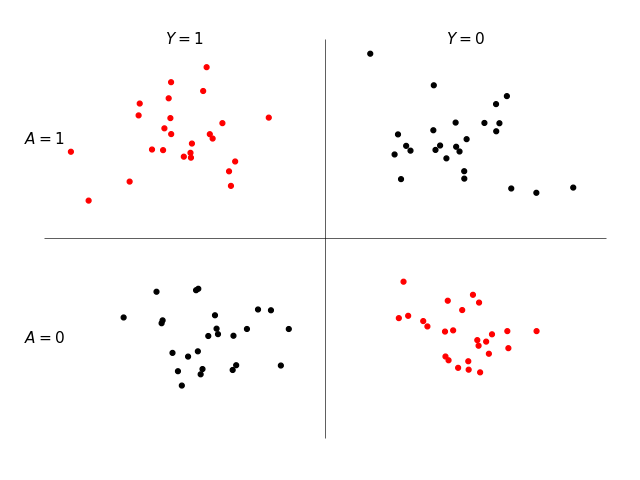
\includegraphics[width=0.8\textwidth]{segadusmaatriks_oigsus.png}
    \end{figure}
\end{frame}
%---------------------------------------------------------

%---------------------------------------------------------
\begin{frame}{Täpsus}
    \begin{figure}[H]
        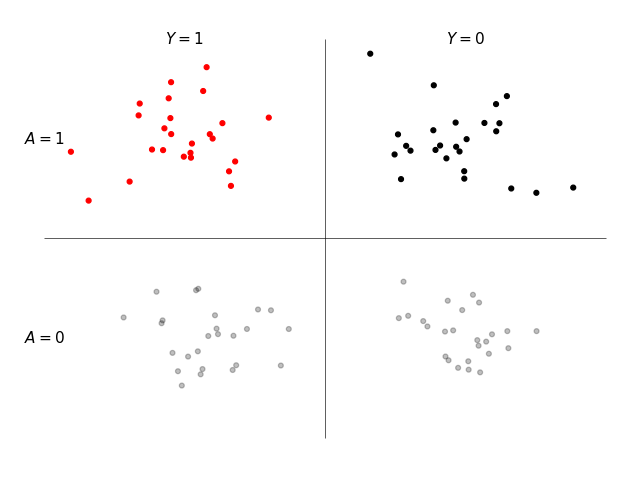
\includegraphics[width=0.8\textwidth]{segadusmaatriks_tapsus.png}
    \end{figure}
\end{frame}
%---------------------------------------------------------

%---------------------------------------------------------
\begin{frame}{Saagis}
    \begin{figure}[H]
        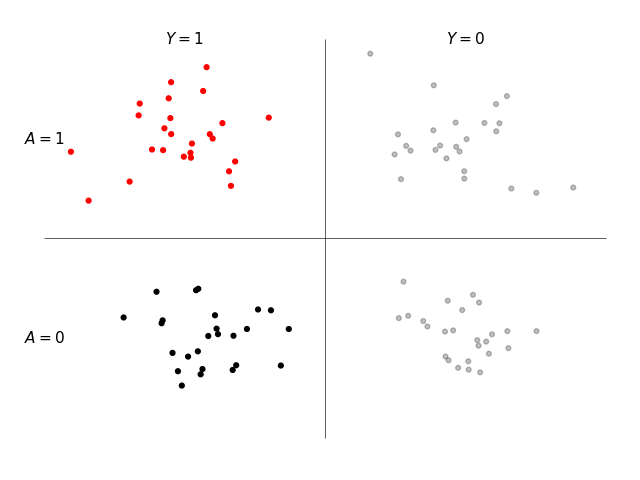
\includegraphics[width=0.8\textwidth]{segadusmaatriks_saagis.png}
    \end{figure}
\end{frame}
%---------------------------------------------------------

%---------------------------------------------------------
\begin{frame}{Konsentratsioonivõrratus}
    \begin{figure}[H]
            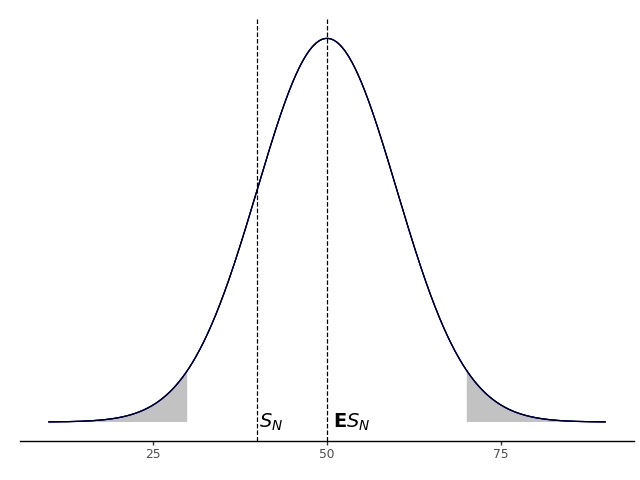
\includegraphics[width=0.7\textwidth]{konsentratsioonivorratus.png}
        \end{figure}
    \begin{equation*}
        S_N = Z_1 + Z_2 + \dots + Z_N , \quad \widehat{\accuracy} = \frac{S_N}{N} , \quad \accuracy = \frac{\mathbf{E} S_N}{N}
    \end{equation*}
\end{frame}
%---------------------------------------------------------

%---------------------------------------------------------
\begin{frame}{Testvalimi suurused}
    \begin{figure}[H]
        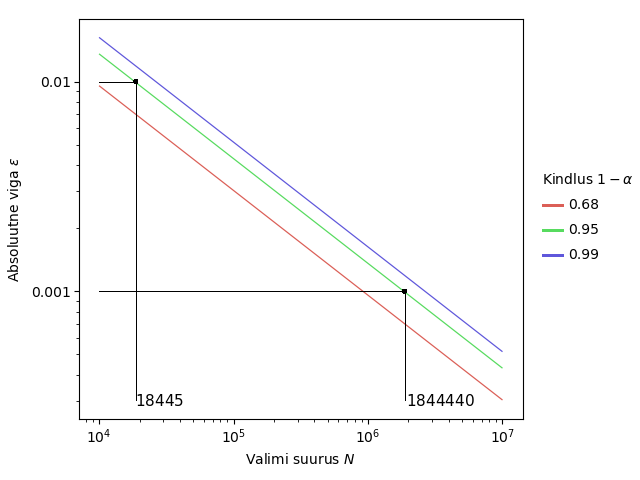
\includegraphics[width=0.8\textwidth]{hoeffding_absoluutne_viga.png}
        \label{fig:höffding absoluutne viga}
    \end{figure}
\end{frame}
%---------------------------------------------------------

%---------------------------------------------------------
\begin{frame}{Testvalimi suurused}
    \begin{figure}[H]
        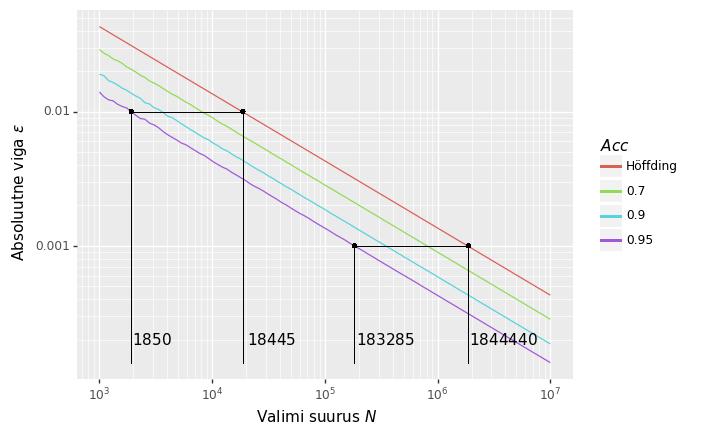
\includegraphics[width=0.8\textwidth]{binoomjaotus_absoluutne_viga.png}
        \label{fig:binoomjaotus absoluutne viga}
    \end{figure}
\end{frame}
%---------------------------------------------------------

\section{Kvaliteedimõõtude võrdlus}

%---------------------------------------------------------
\begin{frame}{Meetodite võrdlus}
    \begin{equation*}
        \Delta \accuracy = \mean{A = Y} - \mean{B = Y} \enspace ,
    \end{equation*}

    Hinnang vahele avaldub andmepunktide kaudu, kus meetodite klassifikatsioonid on erinevad
    \begin{equation*}
        \Delta \widehat{\accuracy} = \frac{1}{N} \cdot \sum_{a_i \neq b_i} [a_i = y_i] - [b_i = y_i] \enspace .
    \end{equation*}

    On võimalik veenduda, kas kaks algoritmi üldse õigsuse poolest erinevad andmepunktide tegelikke klassimärgendeid teadmata
    \begin{equation*}
        \left| \Delta \widehat{\accuracy} \right| \leq \frac{\# \{ i : a_i \neq b_i \}}{N} \enspace .
    \end{equation*}
\end{frame}
%---------------------------------------------------------

%---------------------------------------------------------
\begin{frame}{Meetodite võrdlus}
    \begin{align*}
        \Delta \widehat{\precision} &= \frac{1}{S} \cdot \sum_{a_i \neq b_i} [a_i = 1] \cdot [y_i=1] - [b_i=1] \cdot [y_i=1] \enspace , \\
        \Delta \widehat{\recall} &= \frac{1}{T} \cdot \sum_{a_i \neq b_i} [a_i = 1] \cdot [y_i = 1] - [b_i = 1] \cdot [y_i = 1] \enspace .
    \end{align*}
\end{frame}
%---------------------------------------------------------

%---------------------------------------------------------
\begin{frame}{Vahede lähendid komponenthaavald}
    Lähend vahele on ka leitav komponenthaaval
    \begin{align*}
        \Delta \widehat{\accuracy} &= \hat{\beta} \cdot \hat{\gamma} \enspace ,
    \end{align*}
    millest suuruse $\hat{\beta}$ leidmiseks ei pea andmepunkte märgendama.
\end{frame}
%---------------------------------------------------------

\end{document}